\renewcommand{\thefootnote}{\arabic{footnote}}

\section{Data}

\begin{figure}[tb]
  \centerline{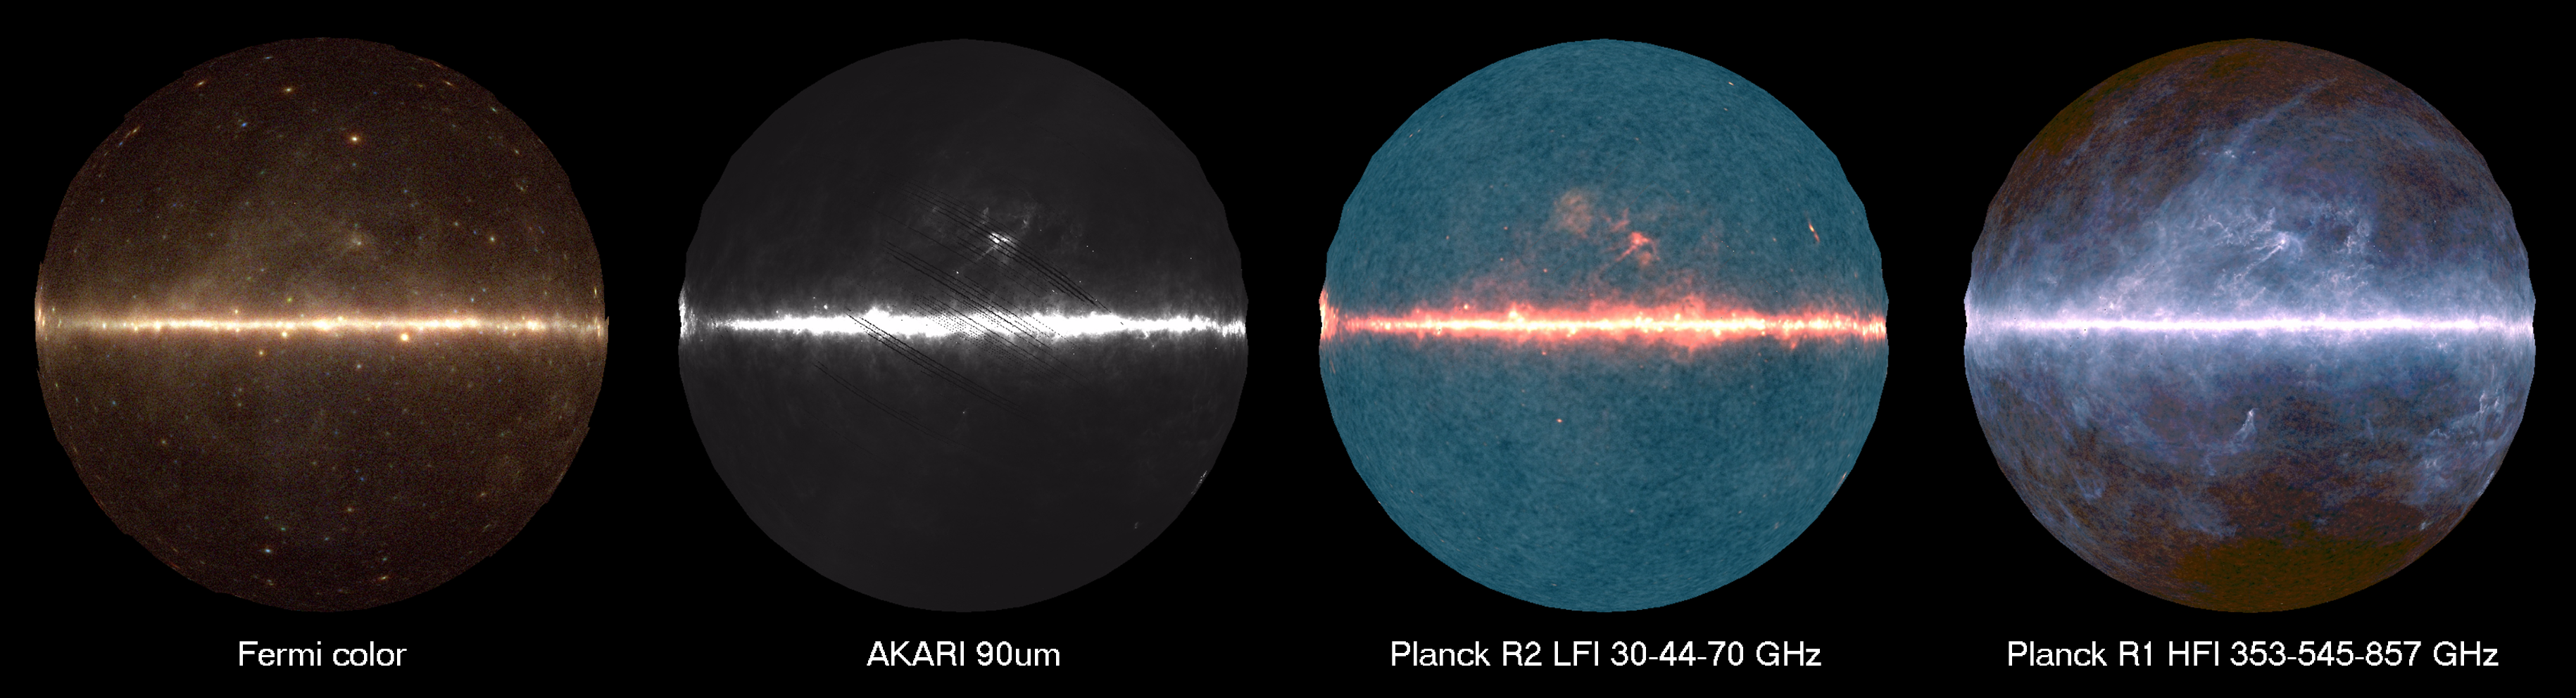
\includegraphics[width=\textwidth]{figures/four_images}}
  \caption{Survey images (left to right): Fermi color, AKARI 90um, Planck LFI, Planck HFI. Images centered on the Galactic Center, FOV 180 degrees.}
  \label{fig:four_images}
\end{figure}

\begin{figure}[tb]
  \centerline{\includegraphics[width=\textwidth]{figures/vela_region}}
  \caption{The Vela Region in various survey images and color maps, FOV 20 degrees.}
  \label{fig:vela_region}
\end{figure}

% \begin{figure}[tb]
%   \centerline{\includegraphics[width=\textwidth]{figures/inner_galaxy_region}}
%   \caption{The inner Galaxy in various survey images and color maps, FOV 45 degrees.}
% \end{figure}

% \begin{figure}[tb]
%   \centerline{\includegraphics[width=\textwidth]{figures/cygnus_region}}
%   \caption{The Cygnus Region in various survey images and color maps, FOV 20 degrees.}
% \end{figure}

% \begin{figure}[tb]
%   \centerline{\includegraphics[width=\textwidth]{figures/lmc_region}}
%   \caption{The Large Magellanic Cloud (LMC) in various survey images and color maps, FOV 10 degrees.}
% \end{figure}

%table

\begin{table}[h]

\caption{Image information.}
\label{tab:a}
\tabcolsep7pt\begin{tabular}{ || lrlll ||}
\hline

\textbf{Image} & \textbf{Resolution (arcsec)} & \textbf{Type} & \textbf{Color?} & \textbf{Description}\\ \hline
\textbf{Fermi color} & 51.53 & gamma-ray & color & Fermi-LAT\\
\textbf{AKARI 90um} & 51.53 & infrared & grayscale & AKARI\\
\textbf{CGPS-VGPS CONT} & 51.53 & radio & grayscale & \\
\textbf{Spitzer GLIMPSE360} & 1.2 & infrared & color & Spitzer \\
\textbf{Haslam 408} & 51.53 & radio & grayscale & 408 MHz\\
\textbf{IRIS Band 4-100um} & 51.53 & infrared & grayscale & IRIS \\
\textbf{Planck R2 LFI Color 30-44-70 GHz} & 51.53 & microwave & color & Planck 30-44-70 GHz\\
\textbf{Planck R1 + R2 HFI Color 353-545-857 GHz} & 51.53 & microwave & color & Planck 353-545-857 GHz\\
\hline
\end{tabular}

\end{table}


% Table
\begin{table}[tb]

\caption{
Source catalogs currently displayed on \gammasky .
We plan to add other catalogs of interest to gamma-ray astronomers in the future,
e.g. the upcoming H.E.S.S. and HAWC TeV source catalogs, or the ATNF pulsar catalog.
}
\label{tab:catalogs}
\tabcolsep7pt\begin{tabular}{ lrll }
\hline
Catalog   & Sources & Updates    & Description \\
\hline
gamma-cat &     153 & continuous & Open TeV gamma-ray source catalog  \\
&&& \gammacat  \\
2FHL      &     360 & fixed      & Second Fermi-LAT catalog of high-energy sources \citep{2fhl}\\
&&& \url{http://fermi.gsfc.nasa.gov/ssc/data/access/lat/2FHL/}  \\
3FGL      &    3034 & fixed      & Third Fermi-LAT point source catalog \citep{3fgl}\\
&&& \url{http://fermi.gsfc.nasa.gov/ssc/data/access/lat/4yr_catalog/}  \\
SNRcat    &     378 & continuous & A census of high-energy observations of Galactic supernova remnants \citep{snrcat}\\
&&& \url{http://www.physics.umanitoba.ca/snr/SNRcat/} \\
\hline
\end{tabular}
\end{table}



The default base image layer displayed on gamma-sky.net's Map View page is a multi-wavelength all-sky survey from Fermi-LAT. In its native color map, source regions appear as certain colors according to their determined energies - red/yellow for 300-1000 MeV, green for 1-3 GeV, and blue for 3-300 GeV. The Fermi color image is presented on the website as a Hierarchical Progressive Survey (HiPS) image \cite{hips}. HiPS is a hierarchical data structure utilizing the HEALPix\footnote[1]{\url{http://healpix.sourceforge.net/}} tesselation of a sphere that organizes data onto pixelated tiles of scalable resolution. The image mechanism allows catalog data and source markers on gamma-sky.net to be visualized accurately on the sky map at various zoom levels. The Centre de Donn\'{e}es astronomiques de Strasbourg (CDS) developed the HiPS technology, and gamma-sky.net currently encompasses 8 survey images also prepared by CDS in this format. The 8 images, which are outlined in Table~\ref{tab:images}, come from CDS's HiPS database\footnote[2]{\url{http://aladin.u-strasbg.fr/hips/list}}, of over 300 prepared HiPS images.

Our website incorporates 4 catalogs which are displayed in Table~\ref{tab:catalogs}. 3FGL \cite{3fgl} and 2FHL \cite{2fhl} are the latest surveys from Fermi-LAT, the main space-based instrument we display sources from. SNRcat \cite{snrcat} is an up-to-date compilation of galactic SNRs observed from a variety of instruments. The database is maintained by the University of Manitoba and can be accessed at \url{http://www.physics.umanitoba.ca/snr/SNRcat/}. gamma-cat is an open-data catalog of sources in the TeV range. As a project that has just recently begun in early September 2016, it is undergoing rapid growth and will be updated frequently on gamma-sky.net. gamma-cat was started at the Max-Planck-Institut f\'{u}r Kernphysik (MPIK) and is open to contribution from other developers. All of its catalog information can be found at \url{https://gammapy.github.io/gamma-cat/}.

User inputs for search fields under the Map View portion of the website are interpreted by the Sesame service\footnote[3]{\url{http://cds.u-strasbg.fr/cgi-bin/Sesame}}. Sesame is a search term resolver for astronomical objects which queries several databases and returns the resolved sources. Both Sesame and the databases searched (SIMBAD, NED, and VizieR) are maintained by CDS.

Under the Catalog View of gamma-sky.net, we are currently showing 3FGL light curve and emission spectrum plots from NASA's Fermi-LAT 3FGL Catalog Interactive Table\footnote[4]{\url{http://fermi.gsfc.nasa.gov/ssc/data/access/lat/4yr_catalog/3FGL-table}}.
